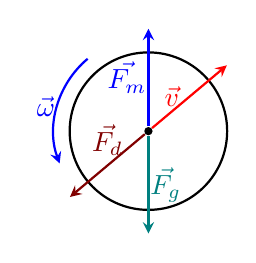
\begin{tikzpicture}
	%giganteska bola de fuego
	\node[fill=black,circle,inner sep=0pt, minimum size=3pt](center) at (0,0)
	{};
 \draw[thick] (center) circle (1);


	%speed
	\draw[thick, red, -stealth] (center) -- node[midway, left] {$\vec{v}$} (40:1.3);

	%gravitace
	\draw[thick, teal, -stealth] (center) --node[midway,right=-3pt] {$\vec{F_g}$} (-90:1.3);

	%drag
	\draw[thick,Maroon, -stealth] (center) --node[midway,left,above] {$\vec{F_d}$}
	 (220:1.3);

	%magnus force
	\draw[thick,blue,-stealth] (center) --node[left=-3pt,midway] {$\vec{F_m}$} (90:1.3);

	%spin
	\draw[thick,blue, -stealth] (130:1.2) arc[
	 start angle = 130,
	 end angle = 200,
	 radius = 1.2
	 ] node[midway,above,left=-3pt] {$\vec{\omega}$};

\end{tikzpicture}
